\documentclass{article}

\usepackage[margin=1in]{geometry}
\usepackage{graphicx} 
\usepackage{gensymb}
\usepackage{amsmath}
\usepackage{multicol}
\usepackage{hyperref}
\usepackage[font=small,labelfont=bf]{caption}

\begin{document}
\begin{titlepage}
    \begin{center}
        \vspace*{1cm}
            
        \Huge
        \textbf{GANs for financial series generation}
            
        \vspace{0.5cm}
        \LARGE
        Use generative adversarial networks to generate financial time series
            
        \vspace{1.5cm}
            
        \textbf{Riccardo Bollati}\\
        \textbf{Elisa Carucci}\\
        \textbf{Stefan Huber}

            
        \vfill
            
        A report presented for the Project course IASP 4090\\
            
        \vspace{0.8cm}
            
        \Large
        The Chinese University of Hong Kong\\
        Hong Kong\\
        09/12/2022
            
    \end{center}
\end{titlepage}


\begin{center}
    {\huge{Introduction}}
\end{center}  
\begin{multicols}{2}
    Financial time series are beneficial for various purposes, for example to train machine learning models or to be used as inputs in market simulators. In these applications, the constraint of limited availability of large amounts of data can have an impact on the performance of the analysis. For these reasons, models, especially deep-learning ones, tend to overfit and struggle at generalizing. By augmenting a dataset we can contribute to the solution of this issue by providing a larger amount of data with respect to what is already accessible. Thanks to this result, companies can effectively  improve models and also use it to enhance strategy backtesting. 
    \subsection*{Characteristics of Time series}
    GANs can capture the temporal structures of financial time-series so as to generate the major stylized facts of price returns, including the linear unpredictability, the fat-tailed distribution, volatility clustering, the leverage effects, the coarse-fine volatility correlation, and the gain/loss asymmetry. 
\end{multicols}    

    \begin{center}
        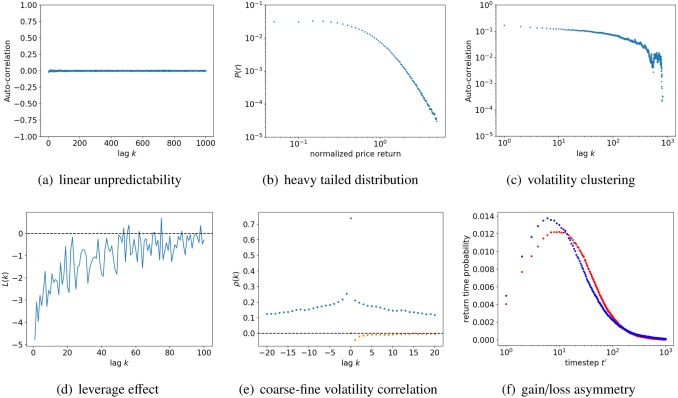
\includegraphics[scale = 0.7]{imgs/elisa/ts.jpg}
    \end{center}
    In the studies of financial time-series, there are two major approaches, namely stochastic processes, and agent-based models, for modeling the financial time-series. However, it is difficult to recover all the major stylized facts with such explicit mathematical formulations. As an alternative approach, GANs have shown spectacular ability in the generation of data including realistic image, audio, natural language text, and financial data.\\
    
\begin{multicols}{2}
    \subsection*{General idea for the data}
    We began by taking a dataset of value stocks from the S\&P 500 as we assumed it would have been easier to analyze financial series with more convenient intrinsic properties such as moderate volatility. In this way it was easier to interpret the results of our model since we could identify out of range peaks very easily. The reasoning behind was due to the fact that it is very hard to judge the performance of a model like this without a defined metric. As for now, we rely on our visual interpretation.\\ 
    
    \subsection*{Scalar method}
    Since the aim of the project is to augment a dataset to be used for further analysis in machine learning, we want to select the generated data that maintain the statistical properties mentioned above. For this reason we will apply a correction algorithm to correct the range of peaks of volatility. We could better observe the results thanks to the choice of our first dataset of stocks with low volatility. It was possible to capture the strange pattern of the series generated since some results did not mimic correctly  the normal behavior of certain types of stocks.\\ 
    
    \subsection*{Further implementation}
   We are now conducting more trials on different types of financial series starting from very volatile stocks. We would like to understand if the performance of the GAN is altered and then explore solutions on how to fix this, if this is the case.  In the future, our next step is to analyze the results of the series obtained with R, to analyze the statistical properties of the series. We would also like to develop a metric to evaluate accurately the performance of the model.\\

    \subsection*{Implementation and Analysis}
    GANs were first used to give images as output so it can be hard to model different kinds of data. In our case we first tried to input prices to get back a financial series that could still preserve the statistical porperties of what we used as input. Unfortunately this was not the case as the series that did not mimic well the real dataset. In fact we can see how the mean was fixed around zero. Of course, there is a mathematical explanation behind this and we will discuss this topic in subsequent chapters.\\
    
    \begin{center}
        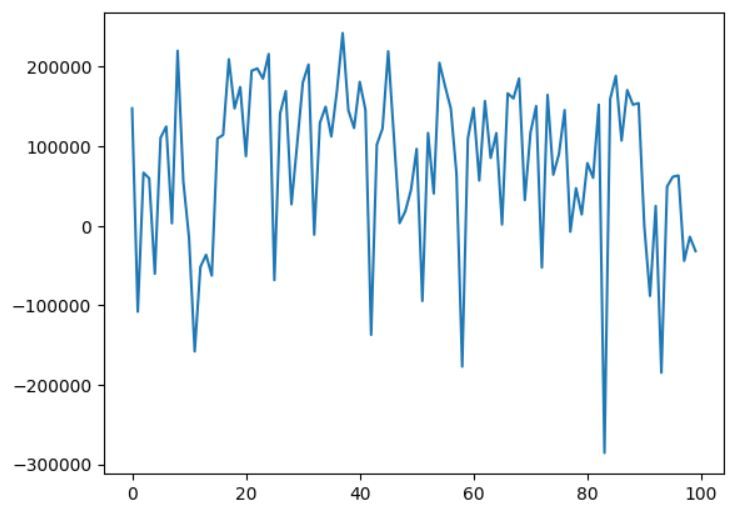
\includegraphics[scale = 0.3]{imgs/elisa/price.jpg}
    \end{center}

    Then, we decided to train the model using net returns which worked and therefore we continued our analysis with these data. As we went on with the implementation of the model, we encountered a problem in terms of randomization.\\

    \begin{center}
        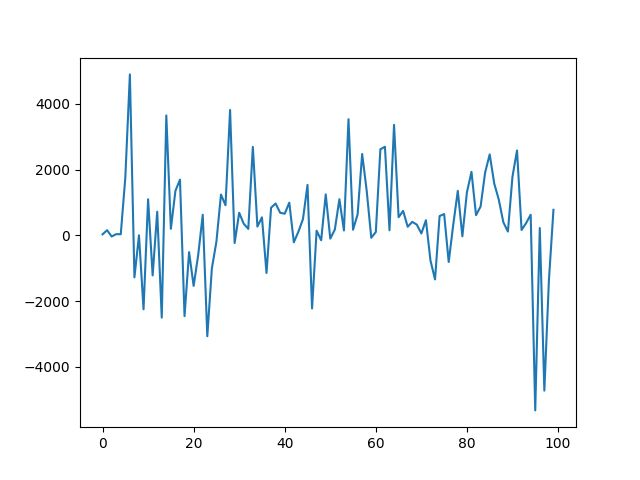
\includegraphics[scale = 0.2]{imgs/elisa/1.jpg}
        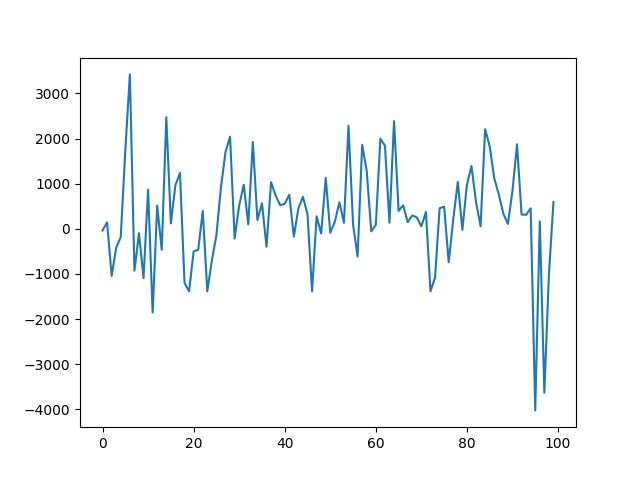
\includegraphics[scale = 0.2]{imgs/elisa/2.jpg}
        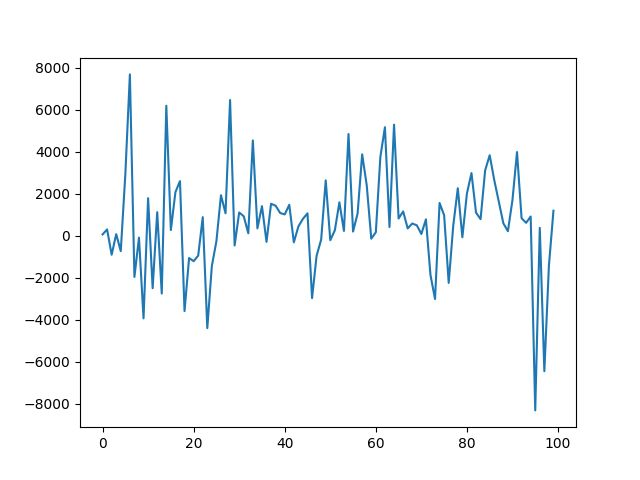
\includegraphics[scale = 0.2]{imgs/elisa/3.jpg}
        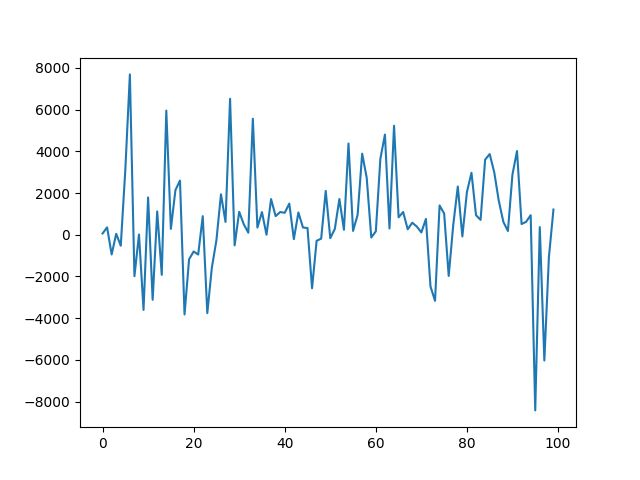
\includegraphics[scale = 0.2]{imgs/elisa/4.jpg}
    \end{center}

    In order to solve this problem we took away the spectral normalization from the generator after doing some trials also with respect to the discriminator. At the end of this process we finally got realistic results which will be shown later in the paper. It is also with these results that we applied the scalar method explained later. \\

    On the other side, we also tried to test the model on log returns with negative results.\\

    \begin{center}
        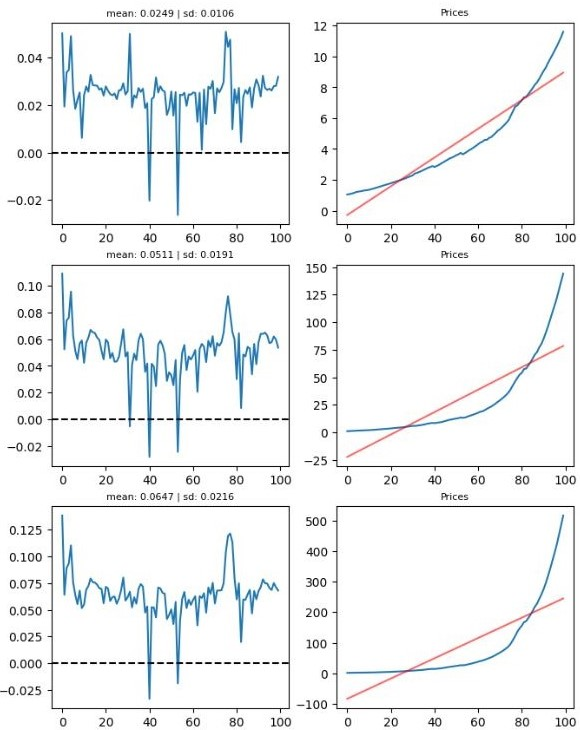
\includegraphics[scale = 0.5]{imgs/elisa/log.jpg}
    \end{center}

    The mean is not around zero as with the net returns. We will now discuss more about these results by comparing the tyoes of returns to be used in financial data analysis.\\

    \subsection*{Returns}
    Prices between assets may be difficult to compare. For example, a large company might have a higher stock price than a smaller competitor. However, the bigger company's price could be relatively stable, while the competitor's smaller price is rapidly increasing. Thus, it is natural to want to think of prices in relative terms. Let's denote the price of an asset at time t. Then the return of an asset captures these relative movements and is defined as:
    $$r_t = \frac{p_t - p_{t-1}}{p_{t-1}}$$
    In words, a return is the change in price of an asset, relative to its previous value. In practice, “returns” often means “log returns”. Log returns are defined as:
    $$z_t = \log(1+r_t)$$
    Returns are lower-bounded by -1.0. One cannot lose more than all of one's money. However, log returns have an infinite support. And since the log function suppresses big positive values while emphasizing small negative values, log returns are more symmetric than returns. This is a natural consequence of logarithms.\\
    In terms of distribution, net returns follow the normal distribution which is symmetric. The lognormal distribution (of log/geometric returns) is not. It's slightly skewed/biased. It happens because the log function is concave around 1, which means it returns "more negative" numbers for values less than 1 than the positive values it returns for numbers the same distance greater than 1. What that means in a practical sense is that when simple returns average zero, log returns are negative, since negative returns have a more negative log return than "equal" positive returns. If your arithmetic mean is positive but close to zero, then it's not unusual to have a small negative log return average. 
    
    \subsection*{Statistical properties of financial time series}
    The final goal related to the implementation of a GAN is to preserve the statistical properties of the data used. We will list the ones that should be used to evaluate the results. Even though we will limit our evaluation to a qualitative visual interpretation, it is our plan to work on accurate mathematical metrics. We list the three main properties. \\
    \subsection*{linear unpredictability}
    The first fundamental property of financial time-series is its linear unpredictability. This property is quantified by the diminishing auto-correlation function of price return. \\
     \begin{center}
        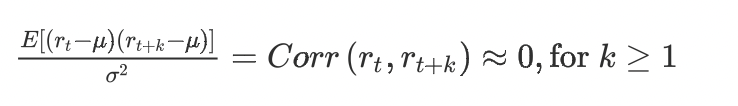
\includegraphics[scale = 0.6]{imgs/elisa/lp.jpg} 
    \end{center}
    The figure shows the decay of the auto-correlation function of the price return in daily scale. The absence of linear correlation in the price return in daily scale implies that the financial markets are efficient to a certain extent.\\
    \subsection*{Fat-tailed distribution}
    The probability distribution has a power-law decay in the tails. A heavy tailed distribution has tails that are heavier than an exponential distribution.  In other words, the tails simply look fatter. As the tails have more bulk, the probability of extreme events is higher compared to the normal. 
    \begin{center}
        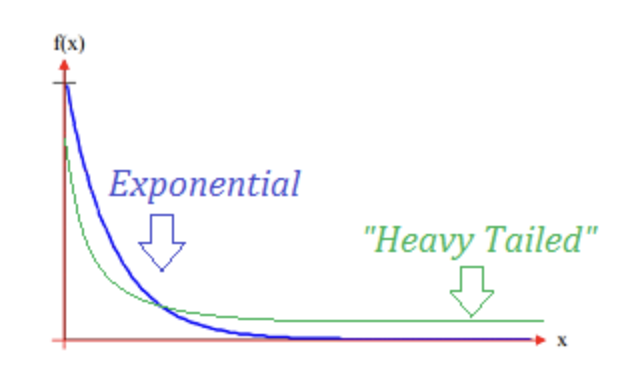
\includegraphics[scale = 0.6]{imgs/elisa/dist.jpg} 
    \end{center}
    

    \subsection*{Volatility clustering}
    While the auto-correlation of the price return is absent, there is still an important temporal structure in the financial time-series, namely volatility clustering. Qualitatively speaking, volatility clustering refers to the fact that the large/small price fluctuations tend to cluster together temporally. Quantitatively, volatility clustering is characterized with the power-law decay of the auto-correlation function of the absolute price returns. 
    \begin{center}
        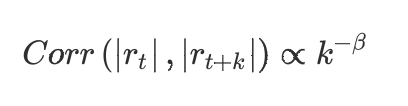
\includegraphics[scale = 0.8]{imgs/elisa/cl.jpg} 
    \end{center}

\end{multicols}


% RICCARDO ------------------------------------------------------------------------------------------------------------------------
\begin{center}
    {\huge{How the Scalar function works}}
\end{center}    
    \begin{multicols}{2}
    The main problem of the data generated by the model is the scale of the data itself.
    As we can see in the following picture, the serie seems realistic if we just look at the trend.
    However, the magnitude of the data is totally out of scale. The algorithm below is designed to force
    the series to converge to the real data range.
    \subsection*{Introduction}
    The scaler aims at scaling the time serie without affecting the trend. The idea is that when we have 
    a peak of returns in the time serie, the significance of the peak depends on its distance from the second highest peak in the serie. For exemple let's take the following series from the dataset of stock values:\\
    \begin{center}
        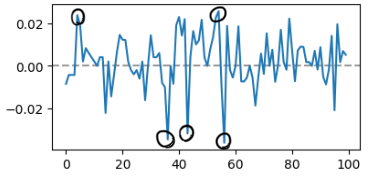
\includegraphics[scale = 0.7]{imgs/riccardo/small_peaks.png}
        \captionof{figure}{}
        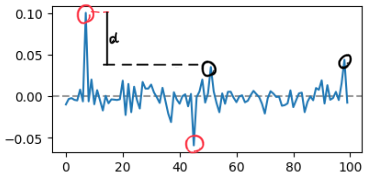
\includegraphics[scale = 0.7]{imgs/riccardo/big_peaks.png}\\
        \captionof{figure}{}
    \end{center}
    As we can see the in (\textbf{Figure 1}) the 2 highest peaks are not very far from each other and that makes the order of magnitude lower compared to the peak we can see in the (\textbf{Figure 2}). Let's analyze two different meanings a peak can refer to:
    \begin{itemize}
        \item a strong movement in price
        \item a shock, due to news or particural events.
    \end{itemize}  
    Taking into consideration the nature of the sample taken, it is very unlikely to have two big shocks in the same window. Following this logic, when the $1^{st}$ and $2^{nd}$ peaks in a serie are close, we can conclude they are probably just strong movements in the price. Again, when the $1^{st}$ peak in terms of magnitude is way bigger than the $2^{nd}$, it is unlinkely to have price movements with this elevated magnitude, in very small ranges. We can note that since the usual price movement of these kind of stocks falls between a range of -0.01\% and 0.01\%, It seems reasonable to apply the scalar function to get an ultimate generated serie that can be used for data analysis purposes while reflecting the true nature of the financial asset. 
    \subsection*{Scalar Logic}
    Based on the above reasonment, the scalar assigns the value that usually shocks have in real data, to isolated peaks in the generated serie, adjusting it to a value plausible in real scenarios.
    It also assigns values typical of strong market movements, to peaks very close to each other.
    \subsection*{Scalar Implementation}
    The scalar computes the quantiles of the max values in the distribution and the same thing for the distribution of the difference between the $1^{st}$ and 
    $2^{nd}$ peaks.\\
    Then, the algorithm takes the sample to see where the distance between the $1^{st}$ and $2^{nd}$ peaks is, among the quantiles of the differences for real 
    data. A random value is then picked from a uniform distribution where the lower and upper bonudaries are the corresponding quantiles in the max distribution. 
    The same is applied to the negative peaks.
    \end{multicols}
    \textbf{Exemple:}
    \begin{center}
        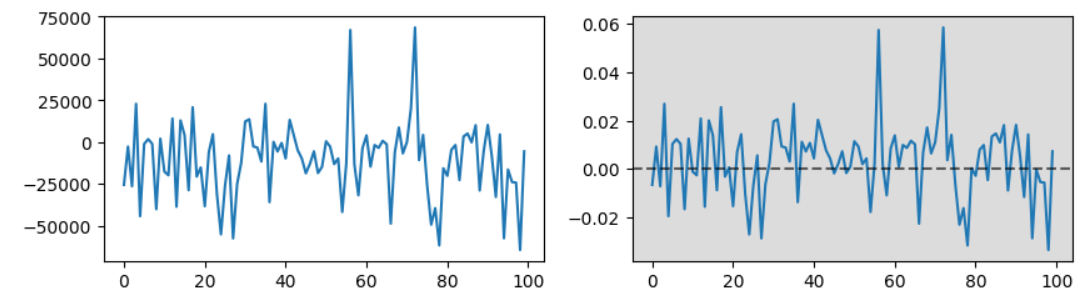
\includegraphics[scale=0.6]{imgs/riccardo/EX_03.png}
    \end{center}
    In the above exemple we can see on the left, the serie generated by our model, and on the rigth the serie after the scaler is applied. As we can see,  
    the scaler preserves the pattern generated by our model and just rescales the data so that we have realistic data we can use for other experiments and implementations.



\begin{center}
    {\huge{Filter}}
\end{center}    
    \begin{multicols}{2}
    \section*{Problem}
    One problem we noticed in the samples generated by our model after the application of the filter is that some are really good and realistic, while others are 
    have no sense, for exemple let's take the samples shwon in the image below:
    \begin{center}
        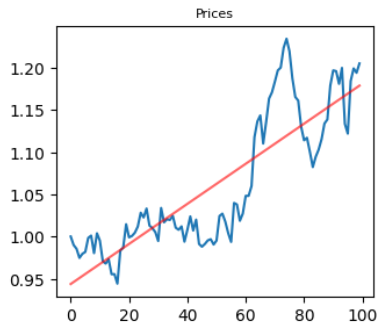
\includegraphics[scale=0.49]{imgs/riccardo/serie_comp_1.png}
        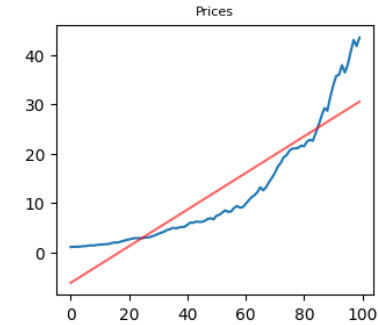
\includegraphics[scale=0.49]{imgs/riccardo/serie_comp_2.png}
    \end{center}
    As we can see, the first series is very realistic while the other one is completly out of scale and shows a trend that is not 
    typical for fiancial time series. In order to solve this problem, we created a filter that selects from the samples generated the realistic series without modifyng the model output, so we end up with a realistic series dataset.
    \section*{How It works}
    To select the realistic series we came up with several metrics, the value of which can be tuned in the filter parameters:
    \paragraph*{Distance between residuals}
    We noticed that once we apply a linear regression to a series, the distance between consecutive residuals is smaller when the series shows an unrelistic behavior.
    In contrast, when we have a more realistic series the discance between consecutive points residuals is bigger.
    \begin{center}
        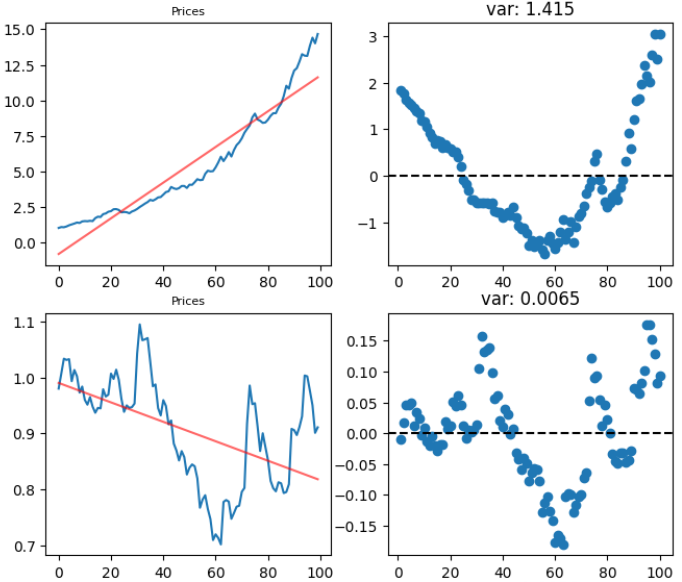
\includegraphics[scale=0.6]{imgs/riccardo/2_res.png}
    \end{center}
    We scaled the price of the generated series between 0 and 1 to make it comparable and applied a linear regression to it. Once we obtained the linear regression, we computed the summation of the distance between consecutive residuals. 
    At this point, the filter just selects the series in which the summation of consecutive residuals is within a given threshold.\\
    \textbf{DfGenerator paramether}:  \textbf{variance\_th}.
    \paragraph*{Maximum range of oscillation}
    We decided to introcuce a parameter in the filter to chose the maximum range of oscillation between the first point an the last one in percentage. This is because we think it could be useful to have the freedom to decide the type of series we want 
    to generate to expand our dataset. Potentially we want to expand our dataset with very volatile series, in this case we can chose to use an hight max range of osscilation. Alternatively, our need could be to expand our dataset with more stable series, for example in order to decrease 
    the volatility of the predictions made by a model. In that case we can tune the parameter chosing a lower max range.\\
    \textbf{DfGenerator paramether}:  \textbf{max\_range}.

    \end{multicols}
    \newpage
    \begin{center}
        {\huge{Final Results}}
    \end{center} 
    The final result of the project is a program capable of generate realistic financial series such the following:
    \begin{center}
        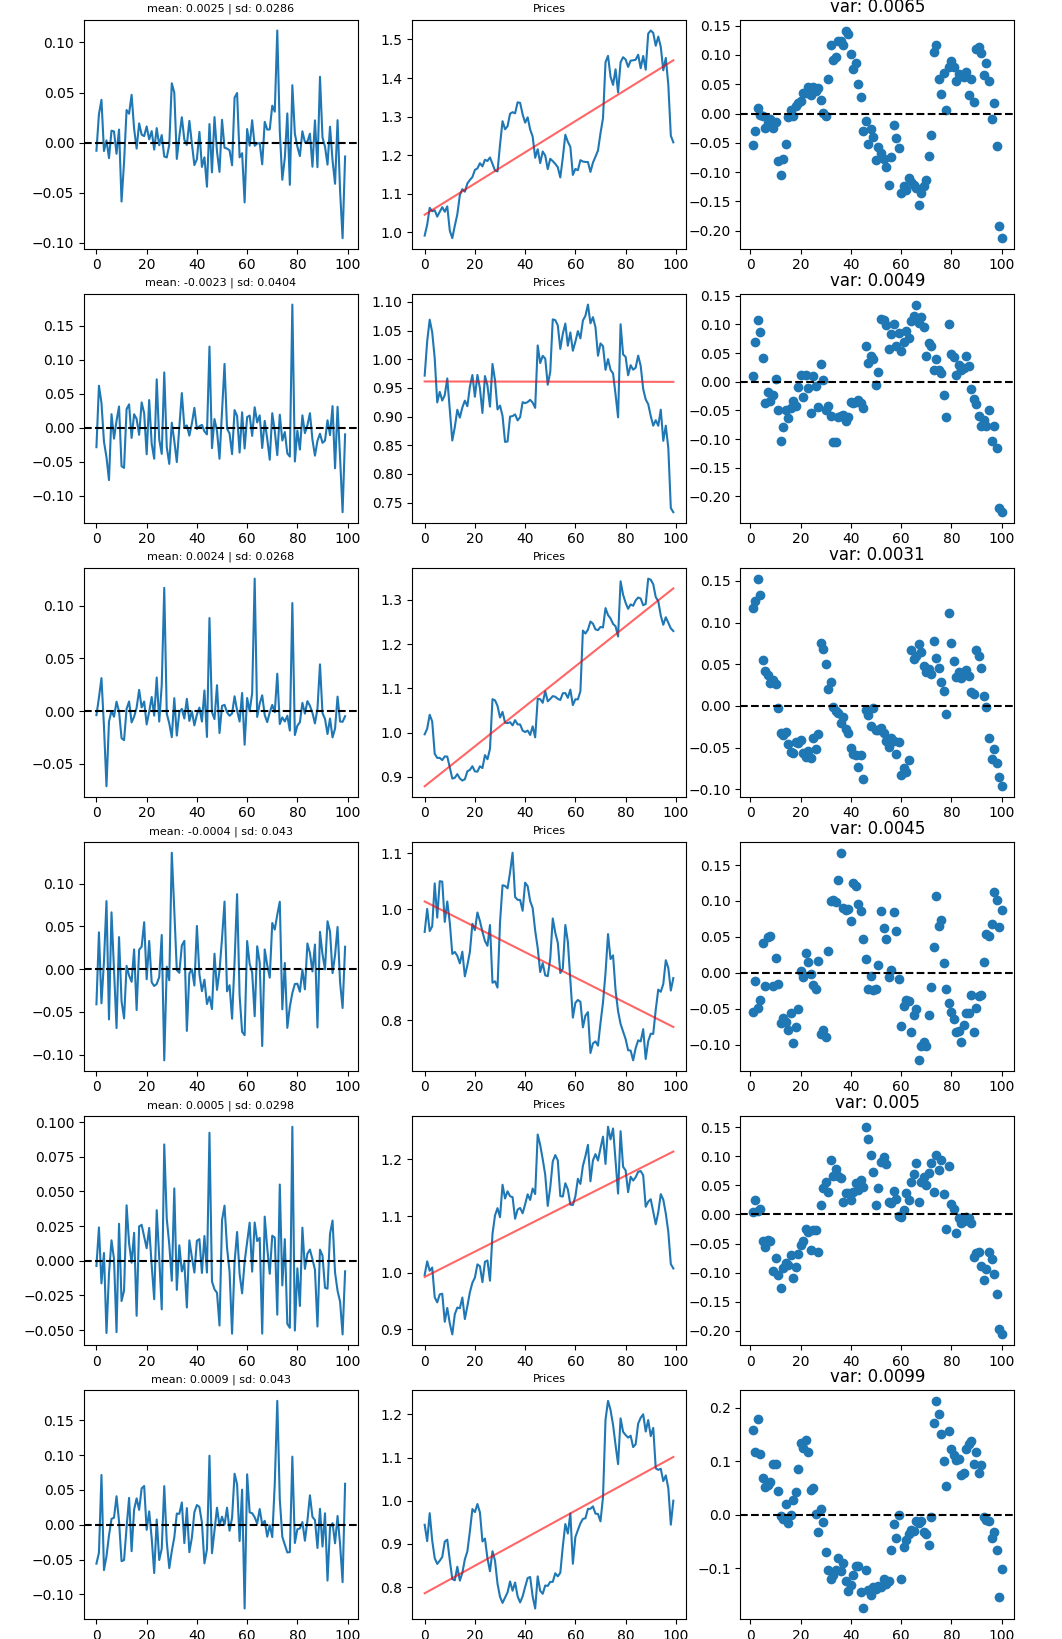
\includegraphics[scale=0.5]{imgs/riccardo/results_reduced.png}
    \end{center}
    \newpage
    The generated series are visually similar to the original series. In the graph, the generated series are represented with a grey background to distinguish them from the original ones:
    \begin{center}
        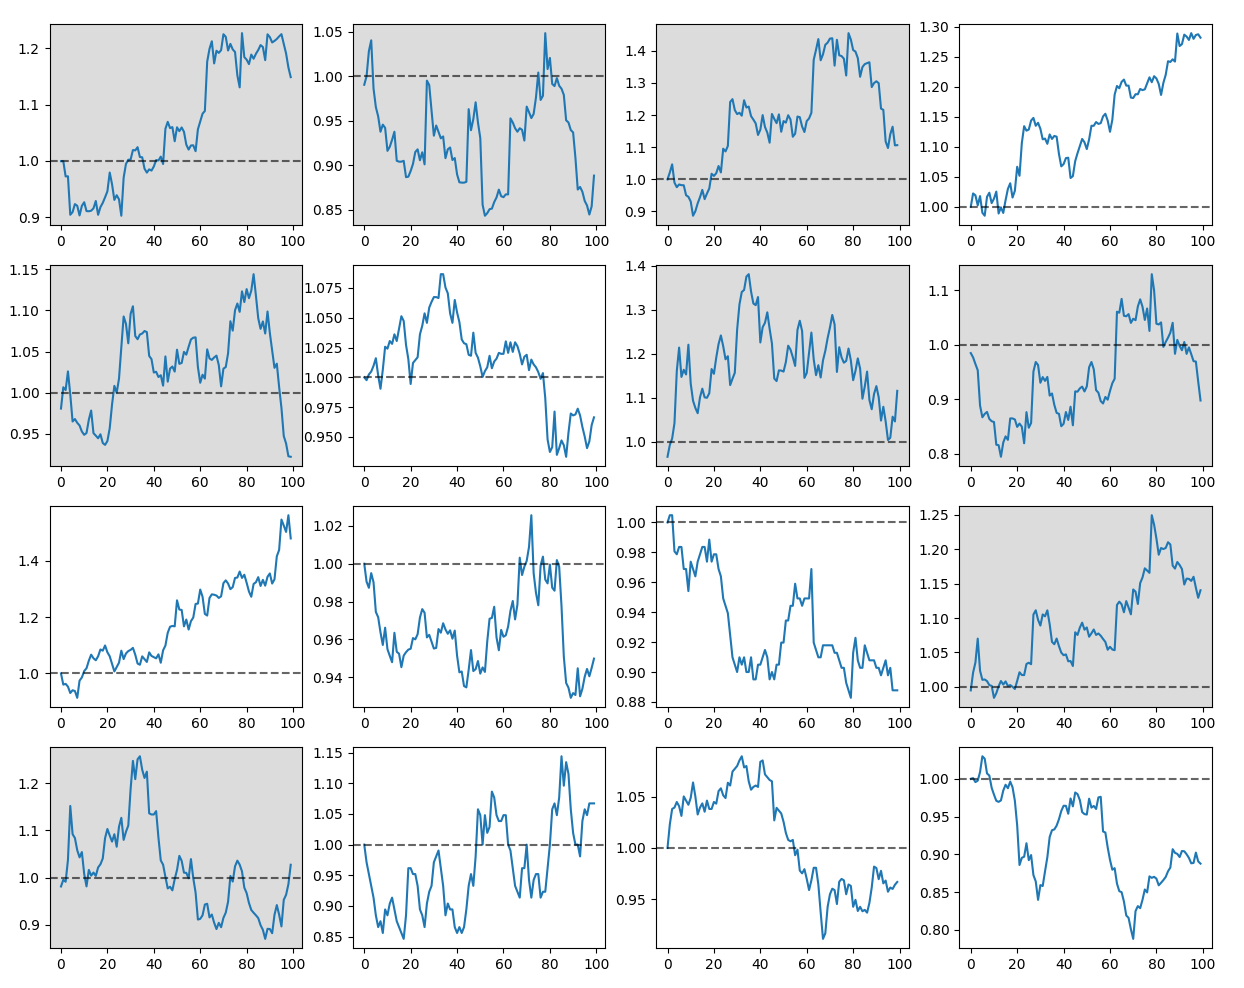
\includegraphics[scale=0.3]{imgs/riccardo/series_comparison_README.png}
    \end{center}
    one of the main characteristic of retuns of financial series is the mean that is almost equal to 0. we generated a dataset of 10 000 samples an computed the mean: 0.00026567.
    The program takes approximatly 20 mintutes to generate a 10 000 samples dataset on a single cpu Intel Core I7. The distribution of the generated samples, looks like this:
    \begin{center}
        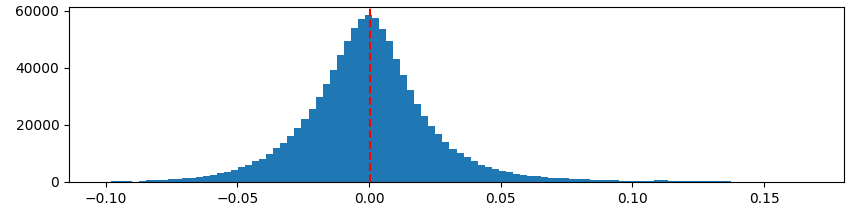
\includegraphics[scale=0.7]{imgs/riccardo/generated.png}
    \end{center}
    
    \newpage
    \begin{center}
        {\huge{Future implementations}}
    \end{center} 
    here we want to briefly want to list some implementation we would like to work on in the Future:
    \begin{enumerate}
        \item Introduction of more rigorous mathematical tests to verify the realisticity of the series generated
        \item try more architectures
        \item implement a tensorboard interface to check models performance realtime during the training
        \item try to inlcude the rescaler in the model architecture of the generator so its paramethers can be optimized during the training
        \item try to feed the model with different types of dataset (e.g. specific sectors stocks) to see how this affect the results
        \item study the statistical properties of the series generated
        \item \textbf{expand a datataset and see how this affect the performances of a prediction model} 
    \end{enumerate}

    % \cite{Mindermann_2022}
    
    \begin{thebibliography}{9}
        \bibitem{citation}
        Mindermann, S., et al. (2022) \emph{Prioritized Training on Points that are learnable, Worth Learning, and Not Yet Learnt.}, \href{https://doi.org/10.48550/arXiv.2206.07137}{arXiv.2206.07.137}.
        
        \bibitem{}

\end{thebibliography}

\end{document}
